\documentclass{beamer}
\usepackage[utf8]{inputenc}
\usepackage{graphicx}

\usetheme{Madrid}
\usecolortheme{whale}

\title{Projet de Programmation Impérative}

\subtitle{K Plus Proches Voisins}

\author{Mathevon B., Palisse E.}

\institute{UJM - L2 Info}

\date{Semestre 4}


\AtBeginSection[]
{
  \begin{frame}
    \frametitle{Table des Matières}
    \tableofcontents[currentsection]
  \end{frame}
}
%------------------------------------------------------------

\begin{document}

\frame{\titlepage}

\begin{frame}
\frametitle{Sommaire}
\tableofcontents
\end{frame}

\begin{frame}{Protocole Expérimental}
Mesure du temps de calcul des KPPV en fonction de deux critères : \\
- Un nombre de K fixe\\
- Un nombre de points fixe
\\
\vskip 1 em
K prend la valeur suivante : k = (2^n)+1 \\
K allant de 1 a n-1 , max = 10000 \\
\vskip 1em
N prend les valeurs suivantes : 10-25-50-100-250-500-1000-5000-10000-50000-100000-500000-1000000\\
\vskip 1em
Pour chaque valeur de N : 10 fichiers aléatoires générés à partir du script data\_gen.sh(nb\_n, nb\_dim, nb\_classe)

\end{frame}

\begin{frame}{Protocole Expérimental}

Pour chaque valeur de n et chaque valeur de k : calcul du temps x10\\
\vskip 1em
Deux méthodes de tris utilisés pour le tableau : \\
-Tri a bulles (O(n²))\\
-Tri fusion (O(n log n))\\
\vskip 1em
Pour le tri a bulles : n max = 10 000\\
Pour le tri fusion : n max = 1 000 000\\
\vskip 1em
Arbre KD (O(log n)) : n max = 1 000 000
\vskip 1em
Calcul de la moyenne pour chaque méthode de tri et chaque valeur de k/n\\
Calcul de l'écart-type (affichage sur les courbes)\\
    
\end{frame}

\begin{frame}{Scripts utilisés}
Temps de calcul : \\
Usage : script\_time.sh\\
\textlangle{}nb\_points\textrangle{}\\
\textlangle{}valeur\_de\_k\textrangle{}\\
\textlangle{}mode(tab/tab\_fusion/arbre)\textrangle{}
\vskip 1em
Moyenne des temps de calcul : \\
Usage: script\_moyenne.sh \\
\textlangle{}type\_moy (en fct de k/n)\textrangle{}\\
\textlangle{}nb\_n si n/nb\_k si k\textrangle{}\\
\textlangle{}mode\textrangle{}
\vskip 1em
Génération d'un graphique : \\
Usage: script\_graph.sh \\
\textlangle{}en fct de n ou k\textrangle{}\\
\textlangle{}valeur de n/k\textrangle{}\\
\end{frame}

\section{K fixe / Nombre de points variables}

\begin{frame}
\frametitle{K fixe}
\begin{columns}
    \column{0.8\textwidth}
    \begin{figure}
      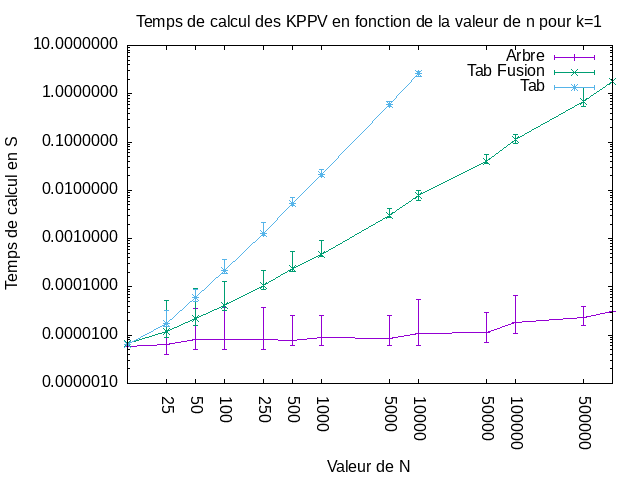
\includegraphics[width=\textwidth]{img_graph/graph_k_1.png}
    \end{figure}
\end{columns}
\end{frame}

\begin{frame}
\frametitle{K fixe}
\begin{columns}
    \column{0.8\textwidth}
    \begin{figure}
      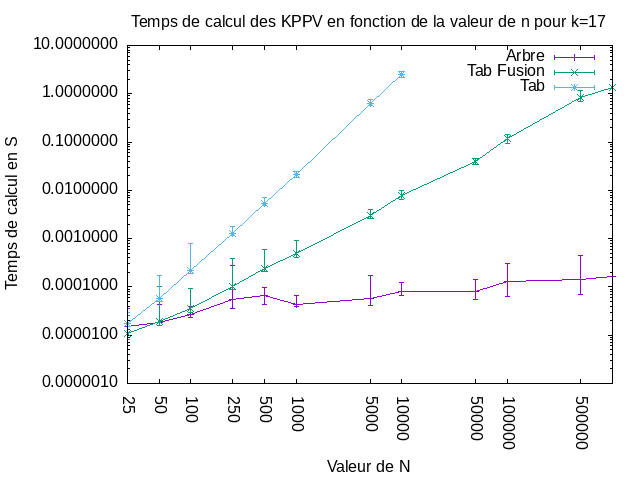
\includegraphics[width=\textwidth]{img_graph/graph_k_17.png}
    \end{figure}
\end{columns}
\end{frame}

\begin{frame}
\frametitle{K fixe}
\begin{columns}
    \column{0.8\textwidth}
    \begin{figure}
      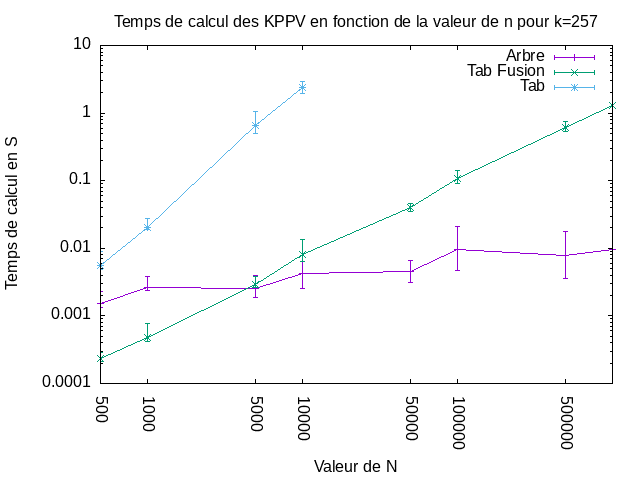
\includegraphics[width=\textwidth]{img_graph/graph_k_257.png}
    \end{figure}
\end{columns}
\end{frame}

\begin{frame}
\frametitle{K fixe}
\begin{columns}
    \column{0.8\textwidth}
    \begin{figure}
      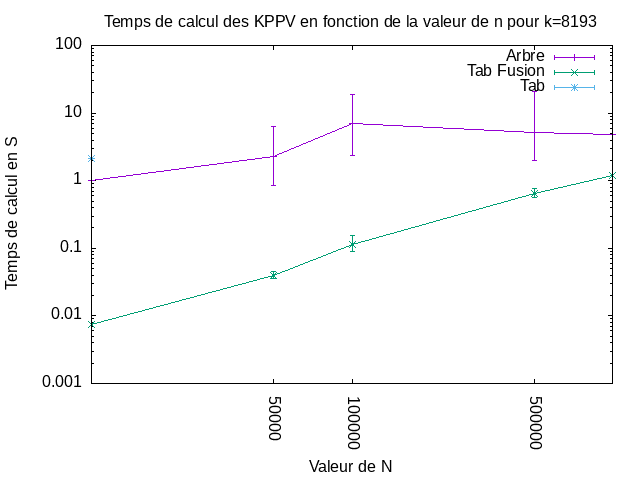
\includegraphics[width=\textwidth]{img_graph/graph_k_8193.png}
    \end{figure}
\end{columns}
\end{frame}

\begin{frame}
\begin{block}{Conclusion K fixe}
Tri par tableau fusion : plus le nombre de points (n) est élevé, plus le temps de calcul augmente.\\
Le temps nécessaire pour trier les données augmente de manière significative lorsque le nombre de points augmente.\\
Méthode moins efficace pour de grands ensembles de données.\\

Méthode par arbre kd : le temps de calcul augmente légèrement avec le nombre de points (n).\\
Temps de calcul toujours plus faible pour un k\textlangle{}10. Donc méthode plus efficace pour un k faible peu importe le nombre de points.\\
Méthode plus efficace pour des ensembles de données plus importants.\\
Mais inversion de la rapidité lorsque le k est très grand.

\end{block}
\end{frame}

\section{Nombre de points fixe / K variable}

\begin{frame}
\frametitle{Nombre de points fixe}
\begin{columns}
    \column{0.8\textwidth}
    \begin{figure}
      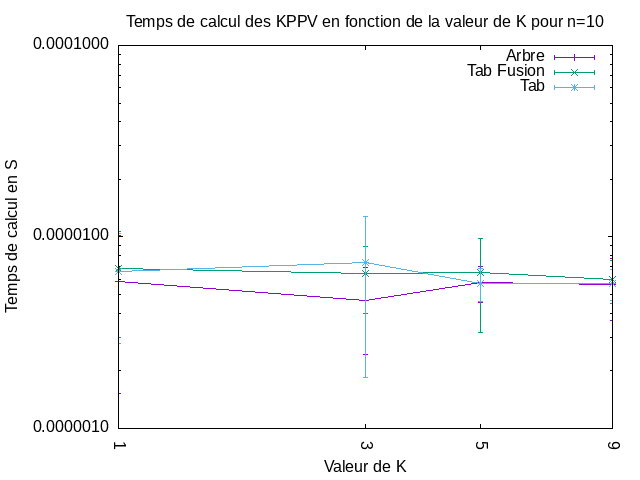
\includegraphics[width=\textwidth]{img_graph/graph_n_10.png}
    \end{figure}
\end{columns}
\end{frame}

\begin{frame}
\frametitle{Nombre de points fixe}
\begin{columns}
    \column{0.8\textwidth}
    \begin{figure}
      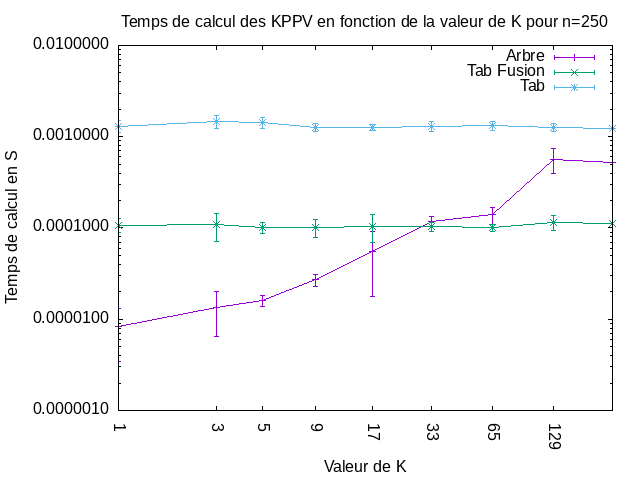
\includegraphics[width=\textwidth]{img_graph/graph_n_250.png}
    \end{figure}
\end{columns}
\end{frame}

\begin{frame}
\frametitle{Nombre de points fixe}
\begin{columns}
    \column{0.8\textwidth}
    \begin{figure}
      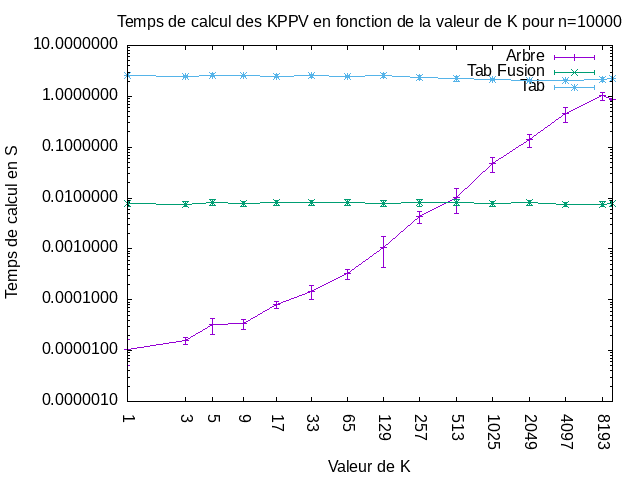
\includegraphics[width=\textwidth]{img_graph/graph_n_10000.png}
    \end{figure}
\end{columns}
\end{frame}

\begin{frame}
\frametitle{Nombre de points fixe}
\begin{columns}
    \column{0.8\textwidth}
    \begin{figure}
      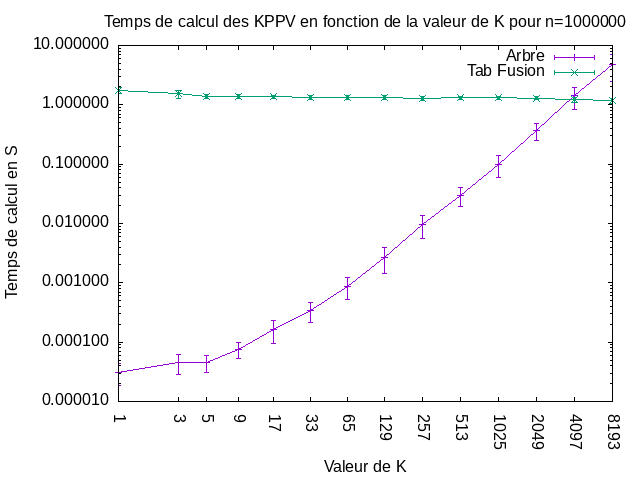
\includegraphics[width=\textwidth]{img_graph/graph_n_1000000.png}
    \end{figure}
\end{columns}
\end{frame}


\begin{frame}
\begin{block}{Conclusion pour nombre de points fixe}
On voit que le temps de calcul par "tableau" reste constant, peu importe la valeur de K.\\
La méthode par arbre kd est plus efficace pour un k relativement faible par rapport au nombre de points.\\
Plus n augmente, plus la valeur de x de l'intersection entre les deux courbes augmente (valeur de k pivot de l'efficacité entre les deux méthodes) car le temps de calcul du tableau augmente.
\end{block}
\end{frame}


\section{ Conclusion }

\begin{frame}
\frametitle{Conclusion}
\begin{itemize}
    \setlength\itemsep{1em}
    \item[{\color{blue}\textbullet}] Pour un k relativement faible par rapport au nombre de points, la méthode par "arbre kd" est plus efficace que la méthode par "tableau". 
    \item[{\color{blue}\textbullet}]Grande valeur de n, faible valeur de k : arbre kd.
    \item[{\color{blue}\textbullet}]Grande valeur de n, grande valeur de k : tableau.
    \item[{\color{blue}\textbullet}]Faible valeur de n, faible valeur de k : arbre kd.
    \item[{\color{blue}\textbullet}]Faible valeur de n, grande valeur de k : tableau.
    \item[{\color{blue}\textbullet}]On voit également sur les courbes que l'écart-type est plus élévé pour la méthode "arbre kd", car fin de parcours de l'arbre plus aléatoire en fonction du placement des points. Donc temps de calcul plus variable que le tableau.
\end{itemize}
\end{frame}

\end{document}

